\documentclass[%
%   preprint,
superscriptaddress,
%groupedaddress,
%unsortedaddress,
%runinaddress,
%frontmatterverbose,
%preprint,
%showpacs,preprintnumbers,
%nofootinbib,
%nobibnotes,
%bibnotes,
%twocolumn,
amsmath,amssymb,
aps,
pre,
%prb,
%rmp,
%prstab,
%prstper,
floatfix,
]{revtex4-2}

\usepackage{graphicx}% Include figure files
\usepackage{overpic}% Include figure files
\usepackage{dcolumn}% Align table columns on decimal point
\usepackage{bm}% bold math
\usepackage{hyperref}% add hypertext capabilities
\usepackage{color}
\usepackage{verbatim}
\graphicspath{{./fig/}}
%\usepackage{epstopdf}
%\usepackage{auto-pst-pdf}

%todo Chris: Write about 1/1 mode
%todo Chris: Write results/figure explanation section

%todo Ralf: Write q_\infty derivation
%todo Ralf: Read and improve introduction. 


\begin{document}
\title{An interactive toy model for the sawtooth oscillation in tokamak fusion reactors}
\author{R.J.J. Mackenbach}
\affiliation{Science and Technology of Nuclear Fusion, Department of Applied Physics, Eindhoven University of Technology, 5600 MB Eindhoven, The Netherlands}
\author{C. B. Smiet}
\affiliation{Princeton Plasma Physics Laboratory, Princeton University, Princeton, New Jersey, USA}
\affiliation{Huygens-Kamerlingh Onnes Laboratory, Leiden University, P.O.\ Box 9504, 2300 RA Leiden, The Netherlands}

\begin{abstract}
  The sawtooth crash is an instability occurring in the core of a tokamak plasma that redistributes the temperature and pressure in the core region.
  In the Kadomtsev model the crash is caused by a 1/1 internal kink that reconnects the hot plasma within the core region.
  In this paper we present a minimal analytical model with two free parameters that reproduces the predicted changes in topology.
  This paints an intuitive picture of how the magnetic topology changes during a sawtooth crash.
\end{abstract}
\maketitle


\section{Introduction}
Global energy consumption keeps increasing, and so do greenhouse gas emissions. This in turn, through many feedback mechanisms \cite{Curry1995,Bloom2010}, raises the earth's average temperature and sea-levels. Since the energy-thirst of the human race is hard to quench, we must turn to renewable energy resources. Many options exist, but only few will be able to sustain the increasing need for energy in the long run. Nuclear fusion, in which small atomic nuclei combine to larger ones releasing vast amounts of energy, is one of those options. 
There are many different concepts for a fusion energy power plant. The tokamak (a Russian acronym for ``\textit{toroidal chamber with magnetic coils}") is the leading candidate as of now (in terms of funding and technological readiness). This doughnut-shaped machine confines a plasma (an ionized gas) by making use of strong magnetic fields and large currents. 
The field in the toroidal direction (long way around the torus) is generated by external coils, while the poloidal field (short way around the tours) that `twists' the field as it goes around is generated by currents in the plasma itself. 
This twisting is quantified by the safety factor $q=n/m$ (where $n$ is the number of toroidal windings of a field line and $m$ the number of poloidal windings).
The plasma contains the fuel of our machine - the deuterium and tritium nuclei which will fuse into helium and produce energy. Using this configuration the tokamak tries to produce more energy than is needed to heat the machine to operating temperature (quantified in Lawson's criterion \cite{Lawson1957}), a feat which ITER hopes to demonstrate.


Tokamaks however, are not free of problems. These machines are plagued by many different complications, such as large heat fluxes and neutron activation of materials. We will focus on one such complication, the sawtooth oscillation. During a sawtooth event, the hot and dense plasma in the core is redistributed through a region in the center of the plasma, causing a sudden drop in the core temperature and density. Slowly, the plasma in the core heats up again and becomes more dense, until the process repeats. If one plots the plasma temperature in the core over time, one would typically see a sawtooth-like pattern, hence the name of the phenomenon.

The sawtooth crash has been observed in tokamak fusion reactors since 1974 \cite{von1974studies, vershkov1974role}.
Because of the temperature dependent Spitzer resistivity, the plasma current that creates the poloidal field in the reactor preferentially concentrates on the hottest plasma region near the magnetic axis.
This decreases the safety factor (increases the twisting) around the core.
Current diffuses onto the core of the tokamak on a slow, resistive timescale, until a fast instability is triggered at a specific value of $q_0$ (the safety factor on the magnetic axis).
This instability leads to mixing of all the plasma in the core, and results in a flat temperature and pressure profile.
It also affects the poloidal and toroidal flux, resulting in a higher $q_0$.
The sawtooth cycle resets, and current slowly accumulates on the axis until the instability is triggered again.

A numerical simulation of a sawtoothing discharge done with M3DC1~\cite{jardin2012multiple} is shown in figure [REF]. [ADD ANIMATED GIF TO PAPER m3dsim.gif]. 
A simulation such as this reproduces the observed phenomena to a degree, but in order to keep the computing resources manageable, many simplifications to the plasma dynamics need to be made. 
The most advanced calculations of the plasma dynamics cost millions of cpu-hours and are run on exascale devices. 
Another approach is to develop analytical models that reduce the complexity of the problem as much as possible, to still reproduce the essential features of the phenomenon. 

\begin{figure}
    \centering
    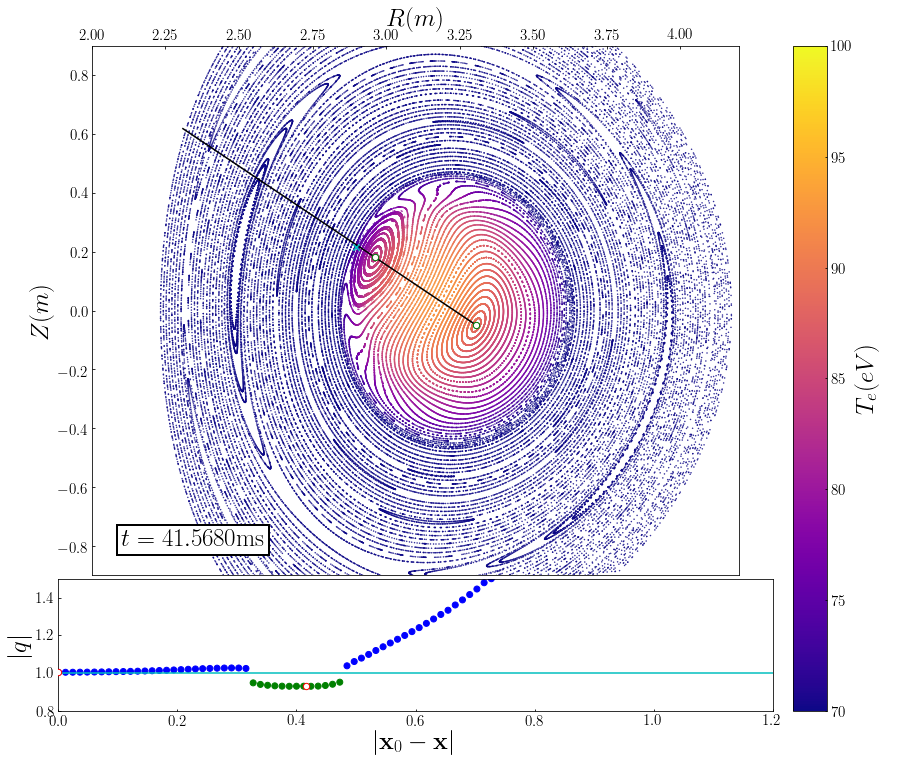
\includegraphics[width=0.7\textwidth]{fullfig149.png}
    \caption{Sawtoothing behavior reproduced in a low-resolution full numerical simulation of plasma dynamics.}
    \label{fig:my_label}
\end{figure}

One of the most enduring models for the sawtooth was presented by Kadomtsev~\cite{kadomtsev1975disruptive}.
In this model the region within the $q=1$ surface becomes susceptible to an internal kink mode, a resistive tearing instability of the $q=1$ surface, or both~\cite{coppi1976resistive}.
The plasma in the core reconnects with cold plasma from outside the $q=1$ surface along a helical ribbon on the $q=1$ surface, and is deposited in a growing 1/1 island.
This growing island eventually completely displaces the hot core, and the temperature and current are redistributed.
After the crash, the hot core is completely replaced by the $1/1$ island, which has $q_0=1$.

In this paper we present a simple analytical toy model that approximates the above process and which uses only  two independent parameters to reproduce the predicted change in topology: a 1/1 internal kink that displaces the core, and a linear interpolation between the initial and final flux predicted by Kadomtsev.
Other expressions for the time-dependent magnetic topology during the sawtooth crash have been presented by Kolesnichenko~\cite{kolesnichenko1996theory} and Jaulmes~\cite{jaulmes2014redistribution}.
These works calculate the intermediate states in the Kadomtsev reconnection process. 
Our model separates the reconnection phase into two separate and independent perturbations, resulting in a more analytically tractable and intuitive picture, at the cost of accuracy.



\section{Theory}

\section*{Initial magnetic field}
The magnetic field in a tokamak ideally consists of nested toroidal magnetic surfaces with a monotonically increasing $q$-profile.
We generate such an equilibrium field using a poloidal flux function $\psi_p(R, Z)$ and a toroidal current function $I(\psi_p)$.
The coordinates used are illustrated in figure~\ref{fig:coords}.
Physically $\psi_p$ represents the amount of flux through the circular disc with radius R centered on the $Z$ axis (indicated by the green circle in figure~\ref{fig:coords}.
$I$, which is sometimes called $F$ or $G$, represents the current through the same surface divided by 2$\pi$.


\begin{figure}\label{fig:coords}
  \begin{overpic}[scale=.5]{fig/torus.png}
    \put(80, 42){\Large $\theta$}
    \put(48, 60){\Large $Z$}
    \put(90, 40){\Large $R$}
    \put(55, 45){\Large $\phi$}
  \end{overpic}
  \caption{Coordinates used for generating the magnetic field. }
\end{figure}

The magnetic fields are calculated from $\psi_p$ and $I$ using:
\begin{equation}\label{eq:unperturbed}
  B_R = -\frac{1}{R} \frac{\partial \psi_p}{\partial Z}, \quad B_z= \frac{1}{R} \frac{\partial
  \psi_p}{\partial R}, \quad
  B_\phi = \frac{1}{R} I.
\end{equation}

For the poloidal flux function we use
\begin{equation}
  \psi_p = a^2,
\end{equation}
where $a=\sqrt{Z^2 + (R-R_0)^2}$ with $R_0$ the location of the equilibrium magnetic axis.
The surfaces of constant $\psi_p$, which are magnetic surfaces, are thus circular-cross-section concentric tori around a magnetic axis located at $R=R_0$.

For our current function $I$ we choose the following relation:
\begin{equation}
  I(\psi) = 2(q_0 + \gamma \psi_p)\sqrt{R_0-\psi_p}.
\end{equation}


The safety factor on each surface is calculated through~\cite{wesson2011tokamaks}:
\begin{equation}\label{eq:qprofint}
  q=\frac{1}{2\pi} \oint \frac{1}{R}\frac{B_\phi}{B_p}\mathrm{d} l,
\end{equation}
where $B_p=\sqrt{B_R^2+B_Z^2}$ is the magnitude of the poloidal magnetic field.
The integration is carried out over a magnetic surface, which in the circular-cross-section concentric toroidal geometry can be done analytically.
The quantity $R B_p$ is constant in this geometry, so we get:
\begin{equation}
  q = \frac{1}{2\pi} \frac{I(\psi_p)}{RB_p}\oint \frac{1}{R} \mathrm{d}l.
\end{equation}
We evaluate the integral by integrating over $\theta$ and using the identities $R=R_0 +a \cos(\theta)$ and $\mathrm{d}l = a \mathrm{d}\theta$ to yield:
\begin{equation}
  \oint \frac{1}{R} \mathrm{d}l = \int_0^{2\pi} \frac{a}{R_0 + a \cos(\theta)} \mathrm{d}l =
  \frac{2\pi a}{\sqrt{R_0^2 -a^2}}
\end{equation}
In the above integration we used the facts that $R_0>0$ and $R_0>a>0$.
This explains our choice of the function $I$, whose square root term cancels against the integrand, giving us the safety factor profile of:
\begin{equation}
  q=q_0 + \gamma \psi_p.
\end{equation}

The expressions in \ref{eq:unperturbed} thus give us an axisymmetric magnetic field where field lines lie on nested concentric toroidal magnetic surfaces with monotonically increasing safety factor.
For this calculation we choose the parameters $\gamma=1$ and $q_0=2/3$.
This field has no Shafranov shift (a shift of the magnetic axis outwards, induced by plasma pressure).
Including a Shafranov shift would make the factor $RB_p$ non-constant on a magnetic surface, thus requiring numerical integration for the evaluation of the integral in~\eqref{eq:qprofint}.

\section*{Internal Kink}
We calculate the change in magnetic field caused by an ideal displacement $\boldsymbol{\xi}$. 
Here $\boldsymbol{\xi}(R, \phi, Z)$ is called the displacement vector that at every point specifies the direction and magnitude of the displacement. 
In linearized ideal MHD, the first order change in magnetic field is given by the expression: 
\begin{equation}\label{eq:kinky}
    \delta \mathbf{B} = \nabla \times (\boldsymbol{\xi} \times \mathbf{B}_0)
\end{equation}
(For those familiar with differential geometry, this expression can be interpreted as the first order effect of Lie dragging the magnetic field in the direction of the displacement vector; $\mathcal{L}_{\boldsymbol{\xi}} \mathbf{B} = \left[\boldsymbol{\xi}, \mathbf{B}\right]$. This reduces to equation~\eqref{eq:kinky} when $\boldsymbol{\xi}$ and $\mathbf{B}$ are divergence free and $\boldsymbol{\xi}$ is infinitesimal.)

The displacement associated with the internal kink is a rigid top-hat displacement of the entire region within the $q=1$ surface. 
At different angles around the torus, the direction varies, making one full rotation around the torus. 
Such a displacement would result in singularities in the perturbed magnetic field when equation~\eqref{eq:kinky} is evaluated. 
These singularities correspond with current sheet formation, but will be troublesome for our numeric integration.

The rigid top-hat displacement of the internal kink has a limiting case that is the marginally stable quasi-interchange mode described by Waelbroeck~\cite{waelbroeck1989nonlinear}. 
This mode occurs when the safety factor is flat and close to 1 in the core region. 
To avoid singularities in our field we opt to implement this smooth displacement function. 

The displacement vector is calculated from a stream function $\Psi$ given by the equation: 
\begin{equation}
    \Psi = e^{-\frac{a^2}{\Delta^2}}\cos(n \phi - m \theta)
\end{equation}
Where $\Delta$ is a characteristic width that limits the extent of the displaced region. 
The displacement is calculated from $\xi_R= -(1/R) (\partial \Psi/\partial z)$ and $\xi_Z= (1/R) (\partial \Psi/\partial R)$. 
The $\phi$-component of the displacement vector is zero. 

As can be seen from equation~\eqref{eq:kinky}, the perturbed field depends on the equilibrium field $\mathbf{B}_0$. 



\section*{The Kadomtsev final state}
We would like to know the final state of the magnetic field after the sawtooth crash. We calculate the predictions of the Kadomtsev model~\cite{kadomtsev1975disruptive} adapting the derivation presented by Biskamp~\cite{Biskamp1997}. Employing the conservation of helical flux $\psi_*$, which is the component of the vector potential in the direction of a helical coordinate, one can find an expression for the final magnetic field. Taking our helical coordinate to be $(1,1)$, the expression for the helical flux in the large aspect ratio limit becomes:
\begin{equation}
    \psi_{*} = (1-q_0)a^2 - \frac{\gamma}{2}a^4.
\end{equation}
This $\psi_*$ has the shape of a ``Mexican hat" potential since $q_0<1$ and $\gamma>0$. The Kadomstev model states that during the crash surfaces inside the $q=1$ surface reconnect with the surfaces outside of the $q=1$ surface. In terms of helical flux, this means that surfaces with equal $\psi_*$ merge with one another.  The surfaces of equal $\psi_*$ can be found by solving the equation
\begin{equation}
    \psi_{*} = C = \text{constant.}
\end{equation}
Solving this equation to $a^2$ will yield two solutions, $a_i^2$ and $a_e^2$, with the property that $a_i^2 < a_e^2$. The final coordinate where the merged surfaces will end up can be found by employing conservation of area between the two merging surfaces,
\begin{equation}
    a_{\infty}^2 = a_e^2 - a_i^2
\end{equation}
Using this, we can find that the helical flux after reconnection becomes
\begin{equation}
    \psi_{*,\infty} = \frac{1}{2}\frac{(1-q_0)^2}{\gamma} - \frac{1}{8} \gamma a^4.
    \label{eq:final-helical-flux}
\end{equation}
Reconnection only occurs when there are two surfaces with equal flux. Otherwise the flux function is unchanged. The last radial coordinate where this reconnection occurs is the mixing radius $a_{\text{mix}}$ , and can be calculated to be
\begin{equation}
    a_{\text{mix}} = \sqrt{ \frac{2(1-q_0)}{\gamma} }.
\end{equation}
Since the toroidal field is mostly generated by the external coils, we expect that the toroidal magnetic field is unchanged. This means that the change in $\psi_*$ comes purely from the poloidal flux function. This results in the final poloidal flux function
\begin{equation}
    \psi_\infty = \begin{cases}
    \frac{3}{8} \gamma a^4 + q_0 a^2 + \frac{1}{2}  \frac{( 1 - q_0  )}{\gamma} , & a<a_{\rm mix} \\
    \psi_p, & a> a_{\rm mix}
    \end{cases}
\end{equation}
from which the magnetic field is calculated in the same way as equation~\eqref{eq:unperturbed}.
One can now also calculate the corresponding safety factor. It is found to be
\begin{equation}
    q_\infty(a) = \begin{cases} 
    \frac{4 \gamma a^2 + 4 q_0}{3 \gamma a^2 + 4 q_0}, & a<a_{\rm mix} \\
    q_0 + \gamma a^2, & a>a_{\rm mix}
    \end{cases}
\end{equation}
This $q$-profile is larger than unity everywhere except at $a=0$, which is as expected. Furthermore, the $q$-profile is discontinuous at $a=a_{\text{mix}}$.


\section{Results}
We construct a Poincar\'e plot of the magnetic field. 
A Poincar\'e plot gives a good sense of the magnetic topology. 
It is calculated by taking a point in the $\phi=0$ plane, numerically calculating the magnetic field line passing through that point, and noting the location where the that field line passes through the $\phi=0$ plane every time it does so. 
If a field line fills out a magnetic surface, and the the field line is followed for long enough, then the Poincar\'e section will start to fill out the circle that corresponds with the intersection of that magnetic surface and the $\phi=0$ plane. 


This procedure is done for 100 different field lines, and each field line is given a different color.
Integration is carried out by a 5th order Runge-kutta method with adaptive step size that runs on a distributed computing network. 
We also calculate the safety factor of each field line, buy counting the number of times it winds around the magnetic axis of the unperturbed field. 
This information is shown below the Poincar\'e plot. 
The Poincar\'e section for the unperturbed field (equation~\eqref{eq:unperturbed}) is visible in figure [REF TO FIG]. 



We can now calculate the total magnetic field, by making use of all our previously calculated functions. The magnetic field takes on the following form:
\begin{equation}\label{eq:totalfield}
    \mathbf{B}_{\text{total}}(\epsilon,\alpha) =  \mathbf{B}_0 + \alpha \mathbf{B}_{1,1}+ \epsilon (\mathbf{B}_\infty -\mathbf{B}_0). 
\end{equation}
The factor $\alpha$ determines the strength of the internal kink perturbation, whereas $\epsilon$ linearly interpolates between the initial state and the final state, as predicted by the Kadomtsev model. 

The effects of these two perturbations on the field can be interactively explored in figure [REF]. 
In figure [REF] different combinations of $\alpha$ and $\epsilon$ can be specifed along a path, and a Poincar\'e plot of every set of ($\alpha$, $\epsilon$) along this path will be computed. 

When a path is chosen such that only $\alpha$ varies, but $\epsilon$ remains zero, we see the effect of the internal kink on the magnetic configuration. 
As can be seen, this results in a shifting of the magnetic axis in the direction of the perturbation, and back again. 

When only $\epsilon$ is varied, but $\alpha$ is kept constant, the magnetic structure does not change at all. 
The only change is seen in the plot of the safety factor, which just linearly interpolates between the initial value of $q_0=2/3$ [change!] and $q_0=0.9$ in the final Kadomtsev state. 

An interesting thing happens when we first apply the internal kink $\alpha$, and with this perturbation in place, start increasing $\epsilon$. 
As soon as $\epsilon$ is non-zero, we see a drastic change in the magnetic structure. 
We see a set of crescent-moon shaped curves in the Poincar\'e plot. 
These are caused by field lines lying on a new type of magnetic surface, that does not surround the magnetic axis anymore. 
Such a structure is called a \emph{magnetic island}. 
Because this structure has appeared on the surface where previously $q=n/m=1/1$, this is called a $1/1$-island. 
Opposite to the center of the island, we see the point where the tips of the crescent moon touch. 
The point where the tips touch exactly is called an X-point. 
There is a field line at the center of the X-point that comes back to itself after one rotation. 

As we continue to increase  $\epsilon$, the size of the island keeps increasing, even when we keep $\alpha$ constant. 
Increasing $\epsilon$ tends to flatten the safety factor profile, bringing $q$ closer to 1 everywhere in the core region.
As $q$ gets closer to 1, it means that field lines rotate around exactly once poloidally per toroidal rotation. 
The perturbation $\mathbf{B}_{1,1}$ given by equation~\eqref{eq:kinky} has exactly the same angular dependence. 
That means that the effect of $\mathbf{B}_{1,1}$ on the trajectory of a field line gets larger and larger, the closer $q$ gets to 1. 
If $\mathbf{B}_{1,1}$ adds a little push to the direction of a field line in one location, it will be adding the same push further along, and at every point, eventually completely changing the trajectory of the field line. 
This effect, where the magnetic structure is strongly affected even by a very small perturbation, if the effect accumulates in this way, is called \emph{magnetic resonance}. 

As we change $\epsilon$ towards 1, the safety factor becomes flatter, and closer to 1. 
This means that the effect of the internal kink becomes stronger, pushing the original magnetic axis further out, and at the same time increasing the size of the island.
When $\epsilon$ gets really close to 1, the original axis gets closer and closer to the X-point, and fewer and field lines surround it, while more and more field lines are part of the island. 
Before $\epsilon$ reaches 1, the effect of the kink is already so strong, that the original axis is pushed into the X-point, and both disappear!

The island has grown so large that it has completely taken over, and the original axis has completely disappeared. 
If we have not returned $\alpha$ to zero, the magnetic field in the core will still be strongly distorted. 
But the drive for such a perturbation has disappeared now that the safety factor is above 1 everyhwere, so the last step should be to return $\alpha$ to 1, and see that the magnetic structure becomes axisymmetric again. 
The final step is to return to the original profile with $q_0<1$, from which the cycle starts anew. 

- fast and slow
- kink triggering
- realistic path

\section*{Conclusions and Discussion}
The model we have presented above gives a very simple intuitive picture of a minimal set of perturbations that result in the topological changes associated with the Kadomtsev sawtooth process. 
We take two effects; the ideal kink and a linear interpolation between two axisymmetric states, to reproduce the changes in magnetic topology that constitute the Kadomtsev satwooth. 


The evolution of the magnetic structure exhibited by our model is probably simpler than what would be physically realized. 
A better approximation would be given by the models presented in~\cite{kolesnichenko1996theory, jaulmes2014redistribution}, as these models give a physical picture for the intermediate states between initial and final state (they for example conserve flux during the process, which the process presented here does not necessarily do). 
Nevertheless, the states in these models will also not correspond exactly to the actual magnetic state during the sawtooth crash, as there will be many other effects present such as current sheet formation, deformation of the shape of the original axis, etc.

\subsection*{Acknowledgements}
We would like to thank H. J. De Blank for enlightening discussions. We would like to thank the entire KingsDS team, D. Desjardins, KC Erb, and P. Navaeiopour, for implementing the model on the distributed computing network. 

\bibliographystyle{naturemag}
\bibliography{refs}

\end{document}
